\documentclass[12pt, a4paper]{article}
\usepackage{cmap} % Улучшенный поиск русских слов в полученном pdf-файле
\usepackage[T2A]{fontenc} % Поддержка русских букв
\usepackage[utf8]{inputenc} % Кодировка utf8
\usepackage[english, russian]{babel} % Языки: русский, английский
\usepackage{enumitem}
\usepackage{pscyr} % Нормальные шрифты
\usepackage{soulutf8}
\usepackage{amsmath}
\usepackage{amsthm}
\usepackage{amssymb}
\usepackage{scrextend}
\usepackage{titling}
\usepackage{indentfirst}
\usepackage{cancel}
\usepackage{soulutf8}
\usepackage{wrapfig}
\usepackage{gensymb}
\usepackage[dvipsnames,table,xcdraw]{xcolor}
\usepackage{tikz}

%Русские символы в списке
\makeatletter
\AddEnumerateCounter{\asbuk}{\russian@alph}{щ}
\makeatother

%Дублирование знаков при переносе
\newcommand*{\hm}[1]{#1\nobreak\discretionary{}%
	{\hbox{$\mathsurround=0pt #1$}}{}}

\usepackage{graphicx}
\graphicspath{{pic/}}
\DeclareGraphicsExtensions{.pdf,.png,.jpg}

%Изменеие параметров листа
\usepackage[left=15mm,right=15mm,
top=2cm,bottom=2cm,bindingoffset=0cm]{geometry}


\usepackage{fancyhdr}
\pagestyle{fancy}
\usepackage{multicol}

\setlength\parindent{1,5em}
\usepackage{indentfirst}

\begin{document}
		
\lhead{Группа 71}
\chead{Модуль 2 Урок 1}
\rhead{Школа <<Симметрия>>}

\section{Введение}
\subsection{Геометрия}
Наука, рассматривающая свойства геометрических фигур, называется \textbf{геометрией}, что в переводе с греческого языка означает \textbf{землемерие}.
Возможно такое название этой науке было дано потому, что в древнее время главной целью геометрии было измерение расстояний и площадей на земной поверхности.

\subsection{Геометрические фигуры}
\textcolor{red}{\textit{Опр.}} Часть пространства, ограниченная со всех сторон, называется \textbf{геометрическим телом}.

\textcolor{red}{\textit{Опр.}} Геометрическое тело отделяется от окружающего пространства \textbf{поверхностью}.

\textcolor{red}{\textit{Опр.}} Часть поверхности отделяется от смежной части \textbf{линией}.

\textcolor{red}{\textit{Опр.}} Часть линии отделяется от смежной части \textbf{точкой}.

Геометрические фигуры могут перемещаться в пространстве, не подвергаясь никаким изменениям.
Две геометрические фигуры называются \textbf{равными}, если перемещением одной из них в пространстве её можно совместить со второй фигурой так, что обе фигуры совместятся во всех своих частях.

\subsection{Плоскость.}
Из различных поверхностей наиболее знакомая нам есть плоская поверхность, или просто \so{плоскость}, представление о которой даёт нам, например, поверхность хорошего оконного стекла или поверхность спокойной воды в пруде.

Укажем следующее \textcolor{red}{\textit{свойство плоскости}}:
\textit{Всякую часть плоскости можно наложить всеми её точками на другое место этой или другой плоскости, причём накладываемую часть можно предварительно перевернуть другой стороной.}

\subsection{Прямая линия}
Самой простой линией является прямая.
Представление о прямой линии, или просто о прямой, всем хорошо знакомо.
Представление о ней даёт туго натянутая нить или луч света, выходящий из малого отверстия.
С этим представлением согласуется следующее основное свойство прямой.

\textcolor{red}{\textit{Свойство прямой:}} \textit{Через всякие две точки пространства можно провести прямую и притом только одну.}

Из этого свойства следует:

\textit{Если две прямые наложены одна на другую так, что какие-нибудь две точки одной прямой совпадают с двумя точками другой прямой, то эти прямые сливаются и во всех остальных точках} (потому что в противном случае через две точки можно было бы провести две различные прямые, что невозможно).

По той же причине \textit{две прямые могут пересечься только в одной точке}.

Прямая линия может лежать на плоскости.
При этом плоскость обладает следующим свойством.

\textcolor{red}{\textit{Свойство плоскости:}} \textit{Если на плоскости взять какие-нибудь две точки и провести через них прямую линию, то все точки этой прямой будут находиться в этой плоскости.}

\subsection{Луч и отрезок}
\textcolor{red}{\textit{Опр.}} Если прямую представляют продолженной в обе стороны бесконечно, то её называют \textbf{бесконечной} (или \textbf{неограниченной}) прямой.

Прямую обозначают обыкновенно двумя большими буквами, поставленными у двух каких-либо её точек.
Так, говорят:
«прямая $AB$» или «$BA$».

\textcolor{red}{\textit{Опр.}} Часть прямой, ограниченная с обеих сторон, называется \textbf{отрезком}.
Отрезок обыкновенно обозначается двумя буквами, поставленными у его концов.
Иногда прямую или отрезок обозначают и одной буквой (малой);
например, говорят: «прямая $a$, отрезок $b$».

Иногда рассматривают прямую, ограниченную только с одной стороны, например в точке $E$.
О~такой прямой говорят, что она исходит из точки $E$;
её называют \textbf{лучом} или \textbf{полупрямой}.

\textcolor{red}{\textit{Опр.}} \textbf{Луч (полупрямая)} — прямая, ограниченная только с одной стороны.


\subsection{Равенство и неравенство отрезков}
\textcolor{red}{\textit{Опр.}} \textit{Два отрезка равны, если они могут быть наложены один на другой так, что их концы совпадут.}

\subsection{Сумма отрезков}
Суммой нескольких данных отрезков $AB$, $CD$, $EF,\dots$ называется такой отрезок, который получится следующим образом.
На какой-нибудь прямой берём произвольную точку $M$ и откладываем от неё отрезок $MN$, равный $AB$, затем от точки $N$ в том же направлении откладываем отрезок $NP$, равный $CD$, и отрезок $PQ$, равный $EF$.
Тогда отрезок $MQ$ и будет суммой отрезков $AB$, $CD$ и $EF$ (которые по отношению к этой сумме называются слагаемыми).
Подобным образом можно получить сумму какого угодно числа отрезков.

Сумма отрезков обладает всеми свойствами суммы чисел;
так, она не зависит от порядка слагаемых (\so{переместительный закон}) и не изменяется, если некоторые слагаемые будут заменены их суммой (\so{сочетательный закон}).
Так:
\[AB+CD+EF=AB+EF+CD=EF+CD+AB=\dots\]
и
\[AB+CD+EF=AB+(CD+EF)=CD+(AB+EF)=\dots\]

\subsection{Действия над отрезками}
Из понятия о сумме выводятся понятия о разности отрезков, умножении и делении отрезков на число.
Так, разность отрезков $AB$ и $CD$ (если $AB>CD$) есть такой третий отрезок, сумма которого с $CD$ равна $AB$;
произведение отрезка $AB$ на число $3$ есть сумма трёх отрезков, из которых каждый равен $AB$;
частное от деления отрезка $AB$ на число $3$ есть третья часть $AB$ и так далее.

Если данные отрезки измерены какой-нибудь линейной единицей (например, сантиметром), и длины их выражены соответствующими числами, то длина суммы отрезков выразится суммой чисел, измеряющих эти отрезки, разность выразится разностью чисел и~т.~д.

\subsection{Окружность}\label{1938/9}
Если дадим циркулю произвольный раствор и, поставив одну его ножку остриём в какую-нибудь точку $O$ плоскости, станем вращать циркуль вокруг этой точки, то другая его ножка, снабжённая карандашом или пером, прикасающимся к плоскости, опишет на плоскости непрерывную линию, все точки которой одинаково удалены от точки $O$.
Эта линия называется \textbf{окружностью}, и точка $O$ — её \textbf{центром}.
Отрезки $OA$, $OB$, $OC,\dots$, соединяющие центр с какими-нибудь точками окружности, называются \textbf{радиусами}.
Все радиусы одной окружности равны между собой.

\begin{wrapfigure}{o}{50 mm}
	\centering
	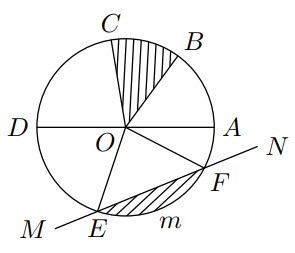
\includegraphics[scale=0.6]{1}
\end{wrapfigure}

Окружности, описанные одинаковыми радиусами, равны, так как они при совмещении их центров совмещаются всеми своими точками.
Прямая, проходящая через какие-нибудь две точки окружности, называется \textbf{секущей}.

Отрезок ($EF$), соединяющий две какие-нибудь точки окружности, называется \textbf{хордой}.

Всякая хорда ($AD$), проходящая через центр, называется \textbf{диаметром}.
Диаметр равен сумме двух радиусов, и потому все диаметры одной окружности равны между собой.
Какая-нибудь часть окружности (например, $EmF$) называется \textbf{дугой}.

О хорде ($EF$), соединяющей концы какой-нибудь дуги, говорят, что она \textbf{стягивает} эту дугу.

Дуга обозначается иногда знаком $\smallsmile$;
например, вместо «дуга $EmF$» пишут «${\smallsmile} EmF$».
Часть плоскости, ограниченная окружностью, называется \textbf{кругом}%
\footnote{Иногда слово «круг» употребляют в том же смысле, как и окружность.
	Но этого следует избегать, так как употребление одного и того же термина для разных понятий может приводить к ошибкам.}%
.

Часть круга, заключённая между двумя радиусами, называется \textbf{сектором}, а часть, отсекаемая от круга какой-нибудь секущей (часть $EmF$), называется \textbf{сегментом}.

\subsection{Равенство и неравенство дуг}\label{1938/10}
Две дуги одной и той же окружности (или равных окружностей) равны между собой, если они могут быть совмещены так, что их концы совпадут.
Допустим, например, что мы накладываем дугу $AB$ на дугу $CD$ так, чтобы точка $A$ совпала с точкой $C$ и дуга $AB$ пошла по дуге $CD$;
если при этом концы $B$ и $D$ совпадут, то совпадут и все промежуточные точки этих дуг, так как они находятся на одинаковом расстоянии от центра, значит, ${\smallsmile} AB={\smallsmile} CD$;
если же $B$ и $D$ не совпадут, то дуги не равны, причём та считается меньше, которая составит часть другой.

\subsection{Сумма дуг}
Суммой нескольких данных дуг одинакового радиуса называется такая дуга того же радиуса, которая составлена из частей, соответственно равных данным дугам.
Так, если от произвольной точки $M$ окружности отложим часть $MN$, равную $AB$, и затем от точки $N$ в том же направлении отложим часть $NP$, равную $CD$, то дуга $MP$ будет суммой дуг $AB$ и $CD$.
Подобно этому можно составить сумму трёх и более дуг.

При сложении дуг одинакового радиуса их сумма может не уместиться на одной окружности, одна из дуг может частично покрыть другую.
В таком случае суммой дуг будет являться дуга, б\'{о}льшая целой окружности.

Сумма дуг, как и сумма отрезков, обладает свойствами \textbf{переместительным} и \textbf{сочетательным}.

Из понятия о сумме дуг выводятся понятия о разности дуг, умножении и делении дуги на число, так же как и для отрезков.

\subsection*{Практика}
\begin{enumerate}
	\item На прямой последовательно откладываются точки $A, B, C, D, E$ и $F$, причем $AB=BC=CD=DE=EF$. Найдите отношения длин отрезков $AD:DF$, $AC:AF$, $BD:CF$
	\item Точка $M$ — середина отрезка $AB$, а точка $N$ — середина отрезка $MB$. Найдите отношения $AM : MN$, $BN : AM$ и $MN : AB$.
	\item Точка $K$ отрезка $AB$, равного $12$, расположена на $5$ ближе к $A$, чем к $B$. Найдите $AK$ и $BK$.
	\item На прямой выбраны четыре точки $A, B, C и D$, причем $AB = 1, BC = 2, CD = 4$. Чему может быть равно $AD$?
	Укажите все возможные варианты.
	\item На линейке отмечены три деления: 0, 2 и 5. Как отложить с ее помощью отрезок длиной 6?
	\item Точка B лежит на отрезке AC длиной 5. Найдите расстояние между серединами отрезков AB и BC.
	\item Даны точки $A$ и $B$. Где на прямой $AB$ расположены точки, расстояние от которых до точки $A$ больше, чем до точки $B$?
	\item Один из двух смежных углов на $30\degree$ больше другого. Найдите эти углы.
	\item Докажите, что биссектрисы двух смежных углов перпендикулярны.
\end{enumerate}

\end{document}